\documentclass{article}

\usepackage{fancyhdr}
\usepackage{extramarks}
\usepackage{amsmath}
\usepackage{amsthm}
\usepackage{amsfonts}
\usepackage{tikz}
\usepackage[plain]{algorithm}
\usepackage{algpseudocode}

\usetikzlibrary{automata,positioning}

%
% Basic Document Settings
%

\topmargin=-0.45in
\evensidemargin=0in
\oddsidemargin=0in
\textwidth=6.5in
\textheight=9.0in
\headsep=0.25in

\linespread{1.1}

\pagestyle{fancy}
\lhead{\hmwkAuthorName}
\chead{\hmwkClass\ (\hmwkClassInstructor\ \hmwkClassTime): \hmwkTitle}
\rhead{\firstxmark}
\lfoot{\lastxmark}
\cfoot{\thepage}

\renewcommand\headrulewidth{0.4pt}
\renewcommand\footrulewidth{0.4pt}

\setlength\parindent{0pt}

%
% Create Problem Sections
%

\newcommand{\enterProblemHeader}[1]{
    \nobreak\extramarks{}{Problem \arabic{#1} continued on next page\ldots}\nobreak{}
    \nobreak\extramarks{Problem \arabic{#1} (continued)}{Problem \arabic{#1} continued on next page\ldots}\nobreak{}
}

\newcommand{\exitProblemHeader}[1]{
    \nobreak\extramarks{Problem \arabic{#1} (continued)}{Problem \arabic{#1} continued on next page\ldots}\nobreak{}
    \stepcounter{#1}
    \nobreak\extramarks{Problem \arabic{#1}}{}\nobreak{}
}

\setcounter{secnumdepth}{0}
\newcounter{partCounter}
\newcounter{homeworkProblemCounter}
\setcounter{homeworkProblemCounter}{1}
\nobreak\extramarks{Problem \arabic{homeworkProblemCounter}}{}\nobreak{}

%
% Homework Problem Environment
%
% This environment takes an optional argument. When given, it will adjust the
% problem counter. This is useful for when the problems given for your
% assignment aren't sequential. See the last 3 problems of this template for an
% example.
%
\newenvironment{homeworkProblem}[1][-1]{
    \ifnum#1>0
        \setcounter{homeworkProblemCounter}{#1}
    \fi
    \section{Problem \arabic{homeworkProblemCounter}}
    \setcounter{partCounter}{1}
    \enterProblemHeader{homeworkProblemCounter}
}{
    \exitProblemHeader{homeworkProblemCounter}
}

%
% Homework Details
%   - Title
%   - Due date
%   - Class
%   - Section/Time
%   - Instructor
%   - Author
%

\newcommand{\hmwkTitle}{Homework 3.2}
\newcommand{\hmwkDueDate}{Feburary 19, 2020}
\newcommand{\hmwkClass}{ENGR 216}
\newcommand{\hmwkClassTime}{Section 509}
\newcommand{\hmwkClassInstructor}{Dr. Ostrovskaya}
\newcommand{\hmwkAuthorName}{\textbf{Amari West}}
\newcommand{\hmwkDueTime}{11:59pm \\ Pages: 15}

%
% Title Page
%

\title{
    \vspace{2in}
    \textmd{\textbf{\hmwkClass:\ \hmwkTitle}}\\
    \normalsize\vspace{0.1in}\small{Due\ on\ \hmwkDueDate\ at \hmwkDueTime}\\
    \vspace{0.1in}\large{\textit{\hmwkClassInstructor\ \hmwkClassTime}}
    \vspace{3in}
}

\author{\hmwkAuthorName}
\date{}

\renewcommand{\part}[1]{\textbf{\large Part \Alph{partCounter}}\stepcounter{partCounter}\\}

%
% Various Helper Commands
%

% Useful for algorithms
\newcommand{\alg}[1]{\textsc{\bfseries \footnotesize #1}}

% For derivatives
\newcommand{\deriv}[1]{\frac{\mathrm{d}}{\mathrm{d}x} (#1)}

% For partial derivatives
\newcommand{\pderiv}[2]{\frac{\partial}{\partial #1} (#2)}

% Integral dx
\newcommand{\dx}{\mathrm{d}x}

% Alias for the Solution section header
\newcommand{\solution}{\textbf{\large Solution}}

% Probability commands: Expectation, Variance, Covariance, Bias
\newcommand{\E}{\mathrm{E}}
\newcommand{\Var}{\mathrm{Var}}
\newcommand{\Cov}{\mathrm{Cov}}
\newcommand{\Bias}{\mathrm{Bias}}

% Allow double underline
\def\doubleunderline#1{\underline{\underline{#1}}}

% Allow for units in math mode
\newcommand{\unit}[1]{\ensuremath{\, \mathrm{#1}}}

\begin{document}

\maketitle

\pagebreak

\begin{homeworkProblem}
	
	A soft-drink machine is regulated so that it discharges an average of 200 millimeters per cup. If the amount of drink is normally distributed with a standard deviation equal to 15 millimeters,
	\\
	
	(a) What fraction of the cups will contain more than 224 millimeters?
	\\ \\
	(b) What is the probability that a cup contains between 191 and 209 millimeters?
	\\ \\
	(c) How many cups will probability overflow if 230 millimeter cups are used for the next 1000 drinks?
	\\ \\
	(d) Below what value do we get the smallest 25\% of the drinks?
	\\ \\
	
	\textbf{\underline{Given}}
	
	\begin{itemize}
		\item $\mu =$ 200 millimeters per cup
		\item $\sigma =$ 15 millimeters
	\end{itemize}
	
	\textbf{\underline{Find}}
	
	\begin{itemize}
		\item The fraction of cups that will contain more than 224 millimeters.
		\item The probability that a cup contains between 191 and 209 millimeters.
		\item The probability that the cups will overflow, assuming 230 millimeter cups are used for the next 1,000 drinks.
		\item The amount at the 25th percentile of drinks.
	\end{itemize}
	
	\textbf{\underline{Diagram}}
	
	\includegraphics[scale=0.90]{problem1.pdf}
	
	\textbf{\underline{Theory}}
	\\
	\\
	To find the probability of a measurement containing a certain value, assuming that the samples follow a normal distribution, the $z$-value must be found with the following equation so that it may be used with the proper $z$-table.
	
	\[
	z = \frac{x - \mu}{\sigma}
	\]
	
	Since under some circumstances the probability may be known but the actual value may be unknown, it's necessary to use the $z$-table and the equation to work backwards and find $x$.
	\\
	
	\textbf{\underline{Assumptions}}
	\\
	
	\begin{itemize}
		\item The curve follows a normal distribution and can be therefore described by $N(200, (15)^2)$
	\end{itemize}

	
	
	\textbf{\underline{Solution}}
	\\
	
	\textbf{Part A}
	\\
	
	First, the $z$ value needs to be calculated using the aforementioned equation.
	
	\[
	\begin{split}
		z &= \frac{224-200}{15}
		\\
		&= 1.6
	\end{split}
	\]
	
	Plug in the value into the $z$-table to get a new value of 0.9452. Take this value and subtract it from 1.0 to get a final answer.
	
	\[
	\begin{split}
		P(x < 224) &= 1 - P(z < 1.6)
		\\
		&= 1 - 0.9452
		\\
		&= \doubleunderline{0.0548}
	\end{split}
	\]
	\\
	
	\textbf{Part B}
	\\
	
	To find the probability that a cup contains between 191 and 209 millimeters, find the $z$-value for the two numbers.
	\\
	First, find $z_1$
	
	\[
	\begin{split}
		z_1 &= \frac{191 - 200}{15}
		\\
		&= -0.6
	\end{split}
	\]
	
	Next, find $z_2$
	
	\[
	\begin{split}
	z_1 &= \frac{209 - 200}{15}
	\\
	&= 0.6
	\end{split}
	\]
	
	Use the $z$-values to find and calculate the probability.
	
	\[
	\begin{split}
		P(191 < x < 209) &= P(-0.6 < z < 0.6)
		\\
		&= P(z < 0.6) - P(z < -0.6)
		\\
		&= 0.7257 - 0.2743
		\\
		&= \doubleunderline{0.4514}
	\end{split}
	\]
	
	\textbf{Part C}
	\\
	
	First, calculate the $z$ value.
	
	\[
	\begin{split}
		z_1 &= \frac{230 - 200}{15}
		\\
		&= 2.0
	\end{split}
	\]
	
	Plug in the value into the $z$-table to get a new value of 2.0. Take this value and subtract it from 1.0 to get the probability.
	
	\[
	\begin{split}
	P(x > 230) &= 1 - P(z > 2.0)
	\\
	&= 1 - 0.9772
	\\
	&= 0.0228
	\end{split}
	\]
	
	Now, multiply the probability by the 1,000 cups used. To find the amount of cups that will overflow.
	
	\[
	\begin{split}
		\unit{Ans} &= (0.0228)(1000)
		\\
		&= \doubleunderline{22.8}
	\end{split}
	\] 
	
	
	\textbf{Part D}
	\\
	
	This problem will need to be worked backwards. Find the number closest to .2500 on the $z$-table to find the corresponding $z$-value which is -0.67. Use the listed equation to find the measurement at the smallest 25\% of drinks or $x$.
	
	\[
	\begin{split}
		\frac{x - 200}{15} &= -0.67
		\\
		x - 200 &= (-0.67)(15)
		\\
		x &= (-0.67)(15) + 200
		\\
		x &= \doubleunderline{189.95}
	\end{split}
	\]
	
	\textbf{\underline{Conclusion}}
	\\
	
	\textbf{Part A}
	\\
	
	The probability that a cup will contain over 224 millimeters is \boxed{5.48\%.}
	\\
	
	\textbf{Part B}
	\\
	
	The probability that a cup will contain between 191 and 209 millimeters is \boxed{45.14\%.}
	\\
	
	\textbf{Part C}
	\\
	
	When rounded, the amount of cups that will overflow is \boxed{23.}
	\\
	
	\textbf{Part D}
	\\
	
	The measurement at the lowest 25\% is \boxed{189.95 \unit{millimeters}.} 
	
\end{homeworkProblem}

\pagebreak

\begin{homeworkProblem}
	
	A lawyer commutes daily from his suburban home to his midtown office. On the average the trip one way takes 24 minutes, with the standard deviation of 3.8 minutes. Assume the distribution of trip times to be normally distributed.
	\\
	
	(a) What is the probability that a trip will take at least 1/2 hour?
	\\ \\
	(b) If the office opens at 9:00 A.M. and he leaves his house at 8:45 A.M. daily, what percentage of the time is he late for work?
	\\ \\
	(c) If he leaves the house at 8:35 A.M. and coffee is served at the office from 8:50 A.M. until 9:00 A.M., what is the probability that he misses coffee?
	\\ \\
	(d) Find the length of time above which we find the slowest 15\% of the trips.
	\\ \\
	(e) Find the possibility that 2 of the next 3 trips will take at least 1/2 hour.
	\\ \\
	
	\textbf{\underline{Given}}
	
	\begin{itemize}
		\item $\mu =$ 24 minutes
		\item $\sigma =$ 3.8 minutes
		\item The lawyer leaves his house at 8:45 A.M.
		\item The office opens at 9 A.M.
		\item Coffee is served from 8:50 A.M. to 9 A.M.
		
	\end{itemize}
	
	\textbf{\underline{Find}}
	
	\begin{itemize}
		\item The probability that a trip takes 1/2 an hour.
		\item The daily percentage that the lawyer is late for work.
		\item The daily probability that the lawyer misses coffee.
		\item The length of time above the slowest 15\% of trips.
		\item The possibility that 2 of the next 3 trips will take at least 1/2 hours.  
	\end{itemize}
	
	\textbf{\underline{Diagram}}
	
	\includegraphics[scale=0.90]{problem2.pdf}
	
	\textbf{\underline{Theory}}
	\\
	
	To find the probability of a measurement containing a certain value, assuming that the samples follow a normal distribution, the $z$-value must be found with the following equation so that it may be used with the proper $z$-table.
	
	\[
		z = \frac{x - \mu}{\sigma}
	\]
	
	Since under some circumstances the probability may be known but the actual value may be unknown, it's necessary to use the $z$-table and the equation to work backwards and find $x$.
	\\
	
	\textbf{\underline{Assumptions}}
	\\
	
	\begin{itemize}
		\item The curve follows a normal distribution and can be therefore described by $N(24, (3.8)^2)$
	\end{itemize}
	
	
	
	\textbf{\underline{Solution}}
	\\
	
	\textbf{Part A}
	\\
	
	First, the $z$ value needs to be calculated using the aforementioned equation.
	
	\[
	\begin{split}
	z &= \frac{30 - 24}{3.8}
	\\
	&= 1.58
	\end{split}
	\]
	
	Plug in the value into the $z$-table to get a new value of 0.9429. Take this value and subtract it from 1.0 to get a final answer.
	
	\[
	\begin{split}
	P(x > 30) &= 1 - P(z > 1.58)
	\\
	&= 1 - 0.9429
	\\
	&= \doubleunderline{0.0571}
	\end{split}
	\]
	
	\textbf{Part B}
	\\
	
	First, the $z$ value needs to be calculated using the aforementioned equation. Since the lawyer is ``late" if he takes over 15 minutes, 15 will be plugged in as $x$.
	
	\[
	\begin{split}
	z &= \frac{15 - 24}{3.8}
	\\
	&= -2.37
	\end{split}
	\]
	
	Plug in the value into the $z$-table to get a new value of 0.0089. Take this value and subtract it from 1.0 to get a final answer.
	
	\[
	\begin{split}
	P(x > 15) &= 1 - P(z > -2.37)
	\\
	&= 1 - 0.0089
	\\
	&= \doubleunderline{0.9911}
	\end{split}
	\]
	
	\textbf{Part C}
	\\
	
	First, the $z$ value needs to be calculated using the aforementioned equation. Since the lawyer is ``late" if he takes over 25 minutes, 25 will be plugged in as $x$.
	
	\[
	\begin{split}
	z &= \frac{25 - 24}{3.8}
	\\
	&= 0.26
	\end{split}
	\]
	
	Plug in the value into the $z$-table to get a new value of 0.6026. Take this value and subtract it from 1.0 to get a final answer.
	
	\[
	\begin{split}
	P(x > 15) &= 1 - P(z > 0.26)
	\\
	&= 1 - 0.6026
	\\
	&= \doubleunderline{0.3974}
	\end{split}
	\]
	
	\textbf{Part D}
	\\
	
	This problem will need to be worked backwards. Find the number closest to .8500 on the $z$-table to find the corresponding $z$-value which is 1.04. Use the listed equation to find the time at the shortest 15\% of trip duration or $x$.
	
	\[
	\begin{split}
	\frac{x - 24}{3.8} &= 1.04
	\\
	x - 24 &= (1.04)(3.8)
	\\
	x &= (1.04)(3.8) + 24
	\\
	x &= \doubleunderline{27.952}
	\end{split}
	\]
	
	\textbf{Part E}
	\\
	
	Using the final answer from Part A, 0.0571, the possibility of the trip taking at least 30 minutes can be found using binomial distribution, as shown.
	
	\[
	\begin{split}
		P(x) &= \frac{n!}{(n - x)!x!} p^x q^{n-x}
		\\
	\end{split}
	\] 
	
	\begin{itemize}
		\item $n$ is the total number of trips
		\item $x$ is the number of trips that last at least 30 minutes
		\item $p$ is 0.0571
		\item $q = p - 1$ is the probability that a trip lasts less than 30 minutes. 
	\end{itemize}

	Now, plug in all of the variables and evaluate.
	
	\[
	\begin{split}
	P(2) &= \frac{3!}{(3 - 2)! \times 2!} (0.0571)^2 (1 - 0.0571)^{3-2}
	\\
	&= \doubleunderline{0.0092}
	\end{split}
	\] 
	
	
	
	\textbf{\underline{Conclusion}}
	\\
	
	\textbf{Part A}
	\\
	
	The probability that the trip will take 30 minutes is \boxed{5.71\%.}
	\\
	
	\textbf{Part B}
	\\
	
	The lawyer is late to work \boxed{99.11\%} of the time.
	\\
	
	\textbf{Part C}
	\\
	
	The lawyer has a \boxed{0.3974\%} chance of being late for coffee.
	\\
	
	\textbf{Part D}
	\\
	
	The slowest trip is \boxed{27.952 \unit{minutes}.}
	\\
	
	\textbf{Part E}
	\\
	
	The possibility that 2 out of the next 3 trips will be at least 30 minutes is \boxed{0.92\%.}
	
	
\end{homeworkProblem}

\pagebreak

\begin{homeworkProblem}
	
	A company pays its employees an average wage of \$9.25 an hour with a standard deviation of 60 cents. If the wages are approximately normally distributed and \underline{paid to the nearest cent},
	\\
	
	(a) What percentage of the workers receive wages between \$8.75 and \$9.69 an hour inclusive?
	\\ \\
	(b) The highest 5\% of the employee hourly wages is greater than what amount?
	\\ \\
	
	\textbf{\underline{Given}}
	
	\begin{itemize}
		\item $\mu =$ \$9.25
		\item $\sigma =$ \$0.60
	\end{itemize}
	
	\textbf{\underline{Find}}
	
	\begin{itemize}
		\item The percentage of workers that receive wages between \$8.75 and \$9.69.
		\item The highest 5\% of the employee hourly wages is greater than what amount?
	\end{itemize}
	
	\textbf{\underline{Diagram}}
	
	\includegraphics[scale=0.90]{problem3.pdf}
	
	\textbf{\underline{Theory}}
	\\
	
	To find the probability of a measurement containing a certain value, assuming that the samples follow a normal distribution, the $z$-value must be found with the following equation so that it may be used with the proper $z$-table.
	
	\[
	z = \frac{x - \mu}{\sigma}
	\]
	
	Since under some circumstances the probability may be known but the actual value may be unknown, it's necessary to use the $z$-table and the equation to work backwards and find $x$.
	\\
	
	\textbf{\underline{Assumptions}}
	\\
	
	\begin{itemize}
		\item The curve follows a normal distribution and can be therefore described by $N(9.25, (0.60)^2)$
	\end{itemize}
	
	
	\textbf{\underline{Solution}}
	\\
	
	\textbf{Part A}
	\\
	
	To find the percentage of workers paid between \$8.75 and \$9.69, find the $z$-value for the two numbers. Since the question asks to round to the nearest cent, round $z_1$ up and $z_2$ down half a cent. Note: the $z$-values here were found using the function \verb|norm| from \verb|scipy.stats| module in python.
	\\
	First, find $z_1$
	
	\[
	\begin{split}
	z_1 &= \frac{8.746 - 9.25}{0.60}
	\\
	&= -0.84
	\end{split}
	\]
	
	Next, find $z_2$
	
	\[
	\begin{split}
	z_2 &= \frac{9.694 - 9.25}{0.60}
	\\
	&= 0.74
	\end{split}
	\]
	
	Use the $z$-values to find and calculate the probability.
	
	\[
	\begin{split}
	P(8.74 \leq x \leq 9.69) &= P(-0.84 \leq z \leq 0.73)
	\\
	&= P(z \leq 0.74) - P(z \leq -0.84)
	\\
	&= 0.7704 - 0.2005
	\\
	&= \doubleunderline{0.5699}
	\end{split}
	\]
	
	\textbf{Part B}
	\\
	
	This problem will need to be worked backwards. Find the number closest to .9500 on the $z$-table to find the corresponding $z$-value which is 1.64. Use the listed equation to find the earnings that mark the top 5\% or $x$.
	
	\[
	\begin{split}
	\frac{x - 9.25}{0.6} &= 1.64
	\\
	x - 9.25 &= (1.64)(0.6)
	\\
	x &= (1.64)(0.6) + 9.25
	\\
	x &= \doubleunderline{10.234}
	\end{split}
	\]
	
	\textbf{\underline{Conclusion}}
	\\
	
	\textbf{Part A}
	\\
	
	The percentage of workers getting paid between \$8.75 and \$9.69 is \boxed{56.99 \%} when rounded to the nearest cent. 
	\\
	
	\textbf{Part B}
	\\
	
	The earnings that mark the top 5\% of hourly wages is \boxed{\$10.23.}
	
\end{homeworkProblem}

\pagebreak

\begin{homeworkProblem}
	
	If a set of observations are normally distributed, what percent of these differ from the mean by
	\\
	
	(a) More than $1.3\sigma$?
	\\ \\
	(b) Less than $0.52\sigma$?
	\\ \\
	
	\textbf{\underline{Given}}
	
	\begin{itemize}
		\item The problem centers around a normal distribution curve
	\end{itemize}

	\textbf{\underline{Find}}
	
	\begin{itemize}
		\item The percentage that is more than $1.3\sigma$
		\item The percentage that is less than $0.52\sigma$ 
	\end{itemize}
	
	\textbf{\underline{Diagram}}
	
	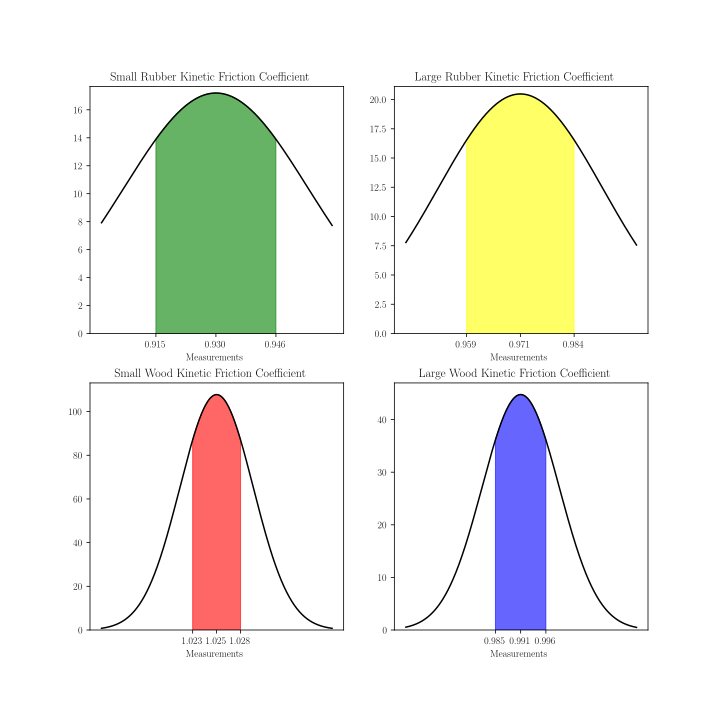
\includegraphics[scale=0.90]{problem4.pdf}
	
	\textbf{\underline{Theory}}
	\\
	
	To find the probability of a measurement containing a certain value, assuming that the samples follow a normal distribution, the $z$-value must be found with the following equation so that it may be used with the proper $z$-table.
	
	\[
	z = \frac{x - \mu}{\sigma}
	\]
	
	Since under some circumstances the probability may be known but the actual value may be unknown, it's necessary to use the $z$-table and the equation to work backwards and find $x$.
	\\
		
	\textbf{\underline{Assumptions}}
	\\
	\begin{itemize}
		\item The curve follows a normal distribution and can be therefore described by $N(0, (1)^2)$
	\end{itemize}
	
	
	\textbf{\underline{Solution}}
	\\
	
	\textbf{Part A}
	\\
	
	First, the $z$ value needs to be calculated using the aforementioned equation. 
	
	\[
	\begin{split}
	z &= \frac{1.3\sigma - 0\sigma}{\sigma}
	\\
	&= 1.3
	\end{split}
	\]
	
	Plug in the value into the $z$-table to get a new value of 0.9032 and plug in the negative value to get 0.0968. Subtract the first value from 1.0 and add the other.
	
	\[
	\begin{split}
	P(x > 1.3) &= 1 - P(z < 1.3) + P(z < -1.3)
	\\
	&= 1 - 0.9032 + 0.0968
	\\
	&= \doubleunderline{0.1936}
	\end{split}
	\]
	
	\textbf{Part B}
	\\
	
	\[
	\begin{split}
	z &= \frac{0.52\sigma - 0\sigma}{\sigma}
	\\
	&= 0.52
	\end{split}
	\]
	
	Plug in the value into the $z$-table to get a new value of 0.6985 and plug in the negative value to get 0.3015. Find the difference between the two values.
	
	\[
	\begin{split}
	P(x > 0.52) &= P(z < 0.52) - P(z < -0.52)
	\\
	&= 0.6985 - 0.3015
	\\
	&= \doubleunderline{0.3970}
	\end{split}
	\]
	
	\textbf{\underline{Conclusion}}
	\\
	
	\textbf{Part A}
	\\
	
	$1.3 \sigma$ differs from the mean by \boxed{19.36\%.}
	\\
	
	\textbf{Part B}
	\\
	
	$0.52 \sigma$ differs from the mean by \boxed{39.7\%.}
	
\end{homeworkProblem}

\pagebreak

\begin{homeworkProblem}
	
	The average life of a certain type of small motor is 10 years with a standard deviation of 2 years. The manufacturer replaces free all motors that fail while under guarantee. If he is willing to replace only 3\% of the motors that fail, how long a guarantee should he offer? Assume that the lives of the motors follow a normal distribution.
	\\
	
	\textbf{\underline{Given}}
	
	\begin{itemize}
		\item $\mu =$ 10 years
		\item $\sigma =$ 2 years
		\item The manufacturer only wants to replace 3\% of motors.
	\end{itemize}
	
	\textbf{\underline{Find}}
	
	\begin{itemize}
		\item How long should the guarantee be if the manufacturer wishes to only replace 3\% of all motors.
	\end{itemize}
	
	\textbf{\underline{Diagram}}
	
	\includegraphics[scale=0.9]{problem5.pdf}
	
	\textbf{\underline{Theory}}
	\\
	
	To find the probability of a measurement containing a certain value, assuming that the samples follow a normal distribution, the $z$-value must be found with the following equation so that it may be used with the proper $z$-table.
	
	\[
	z = \frac{x - \mu}{\sigma}
	\]
	
	Since under some circumstances the probability may be known but the actual value may be unknown, it's necessary to use the $z$-table and the equation to work backwards and find $x$.
	\\
	
	\textbf{\underline{Assumptions}}
	\\
	\begin{itemize}
		\item The curve follows a normal distribution and can be therefore described by $N(10, (2)^2)$
	\end{itemize}
	
	
	\textbf{\underline{Solution}}
	\\
	
	This problem will need to be worked backwards. Find the number closest to .0300 on the $z$-table to find the corresponding $z$-value which is -1.88. Use the listed equation to find 3\% of the motors with the shortest lifespan or $x$.
	
	\[
	\begin{split}
	\frac{x - 10}{2} &= -1.88
	\\
	x - 10 &= (-1.88)(2)
	\\
	x &= (-1.88)(2) + 10
	\\
	x &= \doubleunderline{6.24}
	\end{split}
	\]
	
	\textbf{\underline{Conclusion}}
	\\
	
	The manufacturer warranty should last \boxed{6.24 \unit{years}.}
	
\end{homeworkProblem}

\end{document}
